\documentclass[a4paper,12pt,language=finnish,version=draft,hidechapters=true,includereferences=false,realtimesnewroman=false,sharelatex=false,emptyfirstpages=true]{utuftthesis}
\setcounter{secnumdepth}{2}
\setcounter{tocdepth}{2}

\addbibresource{Bibliografia.bib}
\begin{document}
\begin{comment}
Document template suitable for use as a LaTeX master-file for master's
thesis in University of Turku Department of Future Technologies.\\
\\
Compatible with: ShareLaTeX / PDFLaTeX / XeLaTeX.\\
\\
\\
{*}{*} HOW TO USE? {*}{*}\\
\\
Want to write a thesis? Clone this template in ShareLaTeX or fork
the department's thesis git project.\\
\\
The utuftthesis.cls defines a new thesis class, which is based on
the report class. It supports these new named parameters:

- paper: a4paper

- version: draft / final (default: draft) shows/hides {[}draft{]}
in the header

- language: finnish / english (default: finnish) affects the general
document appearance and hyphenation

- hidechapters: true / false (default: true) hides/shows the chapter/luku
text at the beginning of each Chapter

- includereferences: true / false (default: false) include reference
pages when calculating the total number of pages

- realtimesnewroman: true / false (default: false) use Times New Roman
instead of LaTeX fonts with XeLaTeX. Requires the font to be installed
on the system / provided in the document directory. Other fonts can
be defined with \textbackslash setmainfont.

- sharelatex: true / false (default: false) don't attempt to use (c)
system fonts, instead read them from the project repository

- emptyfirstpages: true / false (default: true) clear the headers/footers
for the 1st pages of text chapters

Traditionally the best places to learn (La)TeX are probably the manual
pages for each package http://www.ctan.org/ and http://www.ctan.org/tex-archive/info/lshort/english/lshort.pdf.
This new version (2.0) should be compatible with xelatex and biblatex
which means that all source files can freely use normal UTF-8 text
without resorting to \textquotedbl\textquotedbl legacy hacks\textquotedbl .\\
\\
Note that PDF/A requirements don't allow PDF links, but if you want
to provide a user friendly version of the thesis with links, use \textbackslash hyperref\\
\\
\\
{*}{*} Maintenance {*}{*}\\
\\
Workflow: https://gitlab.utu.fi/ttweb/thesis -> master .lyx document
exported as .tex documents -> repository content dumped to the sharelatex
project template

Want to fix something in the template? Send a merge.\\
\\
Relies on utuftthesis.cls for the document class definitions.
\end{comment}


\pubyear{2019}
\pubmonth{11}

\pubtype{luk}
\title{Funktionaalisen- ja olioparadigman suorituskykyvertailu Scala-kielessä}
\author{Jaakko Paju}

\maketitle
%
\keywords{suorituskyky, funktionaalinen ohjelmointi, ohjelmointiparadigma, Scala}

\begin{abstract}
Funktionaalisesta ohjelmoinnista lainattuja ominaisuuksia lisätään jatkuvasti perinteisiin imperatiivisiin ohjelmointikieliin. Yksi funktionaalisen ohjelmoinnin keskeisimmistä käsitteistä on muuttumattomat arvot. Muuttumattomien arvojen ja tietorakenteiden käyttö saattaa lisätä kopioimisen tarvetta ja samalla heikentää ohjelman suorituskykyä.

Tutkielman tarkoituksena on perehtyä funktionaalisten ohjelmien suorituskykyyn vaikuttaviin seikkoihin sekä verrata funktionaalisen paradigman suorituskykyä imperatiiviseen paradigmaan. Vertailut tehdään Scala-kielellä, sillä se tukee kumpaakin edellä mainittua paradigmaa. Tutkielmassa keskitytään järjestettyjen muuttumattomien ja muuttuvien kokoelmien suorituskyvyn vertailuun. Suorituskykyä tutkitaan useamman eri mittauksen pohjalta, ja mittauksien tuloksia vertaillaan toisiinsa.

Mittauksissa ei havaittu säännönmukaisia eroja muuttumattomien ja muuttuvien kokoelmien suorituskyvyssä, vaikka muuttuvat kokoelmat olivat joissain mittauksissa hieman muuttumattomia suorituskykyisempiä. Suurin vaikutus suorituskykyyn on tarkoituksenmukaisen tietorakenteen valitsemisella riippumatta onko kyseessä muuttuva vai muuttumaton kokoelma.

Tutkielman pohjalta ei voida tehdä johtopäätöksiä funktionaalisen paradigman kokonaisvaltaisesta vaikutuksesta ohjelman suorituskykyyn. Kokonaisvaltaisten vaikutusten arvioimiseksi tulisi tutkia myös muita funktionaalisen paradigman keskeisiä käsitteitä, kuten sulkeumia, hahmontunnistusta ja rekursiota.
\end{abstract}


% empty pagestyle for table of contents etc.
% otherwise you'll get simple page style with roman page numbers
\pagestyle{empty}

% mandatory
\tableofcontents

% if you want a list of figures
%\listoffigures

% if you want a list of tables
%\listoftables

% 'list of acronyms'
%   - you may not need this at all
%   - create a chapter called List Of Acronyms (or whatever), which
%     should contain all your acronym definitions, e.g. 
%     \chapter{List Of Acronyms} 
%   - the secnumdepth trickery is needed because acronyms are as a
%     standard chapter and we are faking '\listofacronyms'
%
%\setcounter{secnumdepth}{-1}
%\input{your acronym chapter's file name}
%\setcounter{secnumdepth}{2}% setup page numbering, page counter, etc.%
\begin{comment}
The thesis starts here.

To better organize things, create a new tex file for each chapter
and input it below.

Avoid using the å, ä, ö or <space> characters in referred names and
underscores \_ in file names (may break hyperref).

Good luck!
\end{comment}

\chapter{Johdanto} \label{Johdanto}
Funktionaalinen ohjelmointi kasvattaa suosiotaan jatkuvasti. Useisiin yleiskäyttöisiin ja alunperin imperatiivisiin ohjelmointikieliin on lisätty ominaisuuksia funktionaalisesta ohjelmoinnista. Esimerkiksi suositut oliokielet Java, Python ja C++ ovat kaikki lainanneet funktionaalisesta ohjelmoinnista anonyymit sekä korkeamman asteen funktiot.

Funktionaalisen paradigman keskeisistä käsitteitä ovat muuttumattomat arvot ja tietorakenteet. Muuttumattomien arvojen käyttäminen usein lisää kopioimisen tarvetta verrattuna ohjelmiin, joissa käytetään muuttuvia arvoja. Kopioimisen seurauksena muistia pitää varata ja vapauttaa useammin kuin muuttuvia arvoja käytettäessä. Tämä herättää kysymyksen funktionaalisten ohjelmien suorituskyvystä verrattuna imperatiivisiin ohjelmiin.

Tutkielmassa perehdytään tarkastelemaan millaisia vaikutuksia funktionaalisella paradigmalla on suorituskykyyn verrattuna olioparadigmaan. Tutkielman suorituskykyvertailut keskittyvät Scala-ohjelmointikieleen, sillä se on suunniteltu tukemaan sekä funktionaalista että olioparadigmaa, jolloin suorituskyvyn vertailu näiden kahden paradigman välillä on mielekästä ja suoraviivaista. Tarkastelu kohdistuu erityisesti muuttumattomiin kokoelmiin. \todo{Lisää toinen tutkittava aihe} Tutkielma on suoritettu perehtymällä aihetta käsittelevään kirjallisuuteen.

Luvussa \ref{Ohjelmointiparadigmat} esitellään molemmat vertailun kohteena olevat paradigmat. Luvussa \ref{Scala} esitellään Scala-kielen rakenteet, ja miten ne tukevat kumpaakin paradigmaa. Luvussa \ref{Kokoelmat} tarkastellaan Scalan standardikirjaston muuttumattomien kokoelmien suorituskykyä ja verrataan sitä muuttuvien kokoelmien suorituskykyyn. \todo{Varmista että suorituskykyä oikeasti verrataan muuttuviin kokoelmiiin} Viimeisenä luvussa \ref{Yhteenveto} esitellään johtopäätökset ja kootaan tutkielman tulokset.

\todo{Lisää esittely toisesta tutkittavasta aiheesta}

\chapter{Ohjelmointiparadigmat} \label{Ohjelmointiparadigmat}
Ohjelmointiparadigmat luokittelevat ohjelmointikieliä sen perusteella, miten kieli on suunniteltu mallintamaan ongelmia ja minkälaisia mekanismeja kieli tarjoaa näiden ongelmien ratkaisuun. Yhdessä ohjelmointikielessä voi olla vaikutteita useammasta paradigmasta. Tälläistä kieltä kutsutaan \textit{moniparadigmaiseksi} kieleksi. Ohjelmointiparadigmat voi jakaa karkeasti kahteen yläluokkaan: \textit{imperatiivisiin} ja \textit{deklaratiivisiin}.
\cite[Luku 6]{principlesAndParadigms}

Imperatiiviset kielet keskittyvät ohjelmointiongelman ratkaisuun määrittelemällä \textit{miten} tietokoneen tulisi ratkaista laskettava ongelma. Ohjelmat siis rakentuvat peräkkäisistä käskyistä, jotka muokkaavat ohjelman tilaa ja näin ratkaisevat ongelman. Imperatiivisista kielistä puhutaan matalan tason kielinä, sillä ongelman ratkaisu mallinnetaan niissä tietokoneen näkökulmasta.
\cite[Luku 1]{programmingLanguagePragmatics} 

Deklaratiiviset kielet ratkaisevat ongelman vastaamalla kysymykseen \textit{mitä} tietokoneen tulisi tehdä ongelman ratkaisemiseksi. Käytännössä tämä tarkoittaa ongelman ratkaisun kuvailemista ilman toteutuksen yksityiskohtiin uppoutumista. Deklaratiiviset mielletään yleensä korkean tason kielinä, sillä ne mallintavat ongelmanratkaisua ohjelmoijan näkökulmasta.
\cite[Luku 1]{programmingLanguagePragmatics}


\section{Olioparadigma}
Olio-ohjelmoinnnin perusajatus on kuvata ongelmaa olioiden avulla, jotka kukin kuvaavat jotakin ongelma-alueen käsitettä. Olioiden tarkoitus on kapseloida kuvaamansa käsitteen tieto ja tila sisäänsä, sekä tarjota operaatioita kapseloidun tiedon muokkaamiseen ja tarkasteluun. olioparadigma on osa imperatiivisia paradigmoja, sillä ongelmanratkaisu tapahtuu peräkkäisillä komennoilla, jotka muuttavat olioiden ja samalla koko ohjelman tilaa kohti ratkaistua ongelmaa. \cite[Luku 1]{programmingLanguagePragmatics}
\cite[Luku 10]{principlesAndParadigms}


\section{Funktionaalinen paradigma}
Funktionaaliset ohjelmat rakentuvat yksittäisistä funktiosta, joita yhdistämällä luodaan yhä isompia funktiota. Näillä funktioilla ei ole tilaa, ja ne ovat puhtaita eli eivät aiheuta \textit{sivuvaikutuksia}. Sivuvaikutuksia voivat olla esimerkiksi muuttujan arvon muuttaminen, poikkeuksen nostaminen, tiedoston lukeminen tai kirjoittaminen, pyyntö tietokantaan tai verkon ylitse sekä näytölle piirtäminen. Tilaton ja puhdas funktio palauttaa tilanteesta riippumatta tietyllä syötteellä aina saman arvon. \cite[Luku 1]{functionalProgrammingInScala}

Ohjelmointikieli ilman sivuvaikutuksia olisi käytännössä hyödytön, joten funktionaaliset ohjelmointikielet tarjoavat erilaisia mekanismeja sivuvaikutusten hallintaan.  Funktionaalisen ohjelmoinnin katsotaan yleensä kuuluvan deklaratiiviseen paradigmaan. \cite[Luku 11]{principlesAndParadigms}


\section{Paradigmoille tyypillisiä ominaisuuksia}
Lauseke on ohjelmointikielen rakenne, jonka suoritus tuottaa arvon. Lauseke voi koostua joko arvosta tai operaattorista, jota on sovellettu yhteen tai useampaan lausekkeeseen. Esimerkiksi \code{3+2} on numeerinen lauseke, jossa on yksi operaattori \code{+}, jota sovelletaan kahteen numeeriseen arvoon \code{3} ja \code{2}. Lausekkeen arvo voidaan sijoittaa muuttujaan, antaa parametriksi funktioon tai sen arvo voidaan palauttaa funktiosta. Lauseke on minkä tahansa ohjelmointikielen perusrakenne, eli lausekkeita on funktionaalisissa sekä oliokielissä.
\cite[Luku 6]{principlesAndParadigms}

Funktionaalisessa ja olioparadigmassa molemmissa on muuttujia, mutta niitä käsitellään eri tavoilla. Funktionaalisissa kielissä muuttujaan sijoitettua arvoa ei voi muuttaa alustuksen jälkeen, kun taas imperatiivissa kielissä muuttujan arvoa voi yleensä muuttaa. Sama pätee tietorakenteisiin: imperatiivisssa kielissä niiden muuttaminen alustamisen jälkeen on sallittua, funktionaalisissa ei. \cite[Luku 3]{functionalProgrammingInScala} Funktionaalisissa kielissä funktioita kohdellaan kuin mitä tahansa muitakin arvoja: niitä voi sijoittaa muuttujiin, antaa parametrina toiseen funktioon tai käyttää funktion palautusarvona. Oliokielissä tämä ei aina ole mahdollista.
\cite[Luku 6]{principlesAndParadigms}

Komento on ohjelmointikielen rakenne, jonka suoritus ei aina tuota arvoa ja saattaa aiheuttaa sivuvaikutuksia. Komennot saattavat esimerkiksi muuttaa olioiden ja muuttujien tilaa, lukea käyttäjän tuottamaa syötettä tai nostaa poikkeuksen. Komentojen suorittamisella saattaa olla sivuvaikutuksia, joten niiden suoritusjärjestys on merkityksellinen. Imperatiivisiin kieliin komennot kuuluvat oleellisesti, mutta funktionaalisiin eivät.

Imperatiivisissa kielissä toisto toteutetaan silmukoilla. Silmukkaa suoritetaan ennalta määritelty määrä tai kunnes silmukan suoritusta säätelevä ehtolause muuttuu epätodeksi. Ehtolauseen arvo määräytyy muuttujan arvon mukaan, jota muutetaan silmukan suorituksen aikana. Funktionaalisissa kielissä muuttujien arvoa ei voi muuttaa, ja siitä syystä silmukat olisivat hyödyttömiä. Silmukoiden sijaan käytetään rekursiota, eli funktio kutsuu itseään kunnes funktioon määritelty perustapaus saavutetaan.
\cite[Luku 6 ja 11]{principlesAndParadigms}

Kummankin paradigman ominaisuuksissa on omat ongelmakohtansa. Imperatiivisia ohjelmia on tavallisesti vaikea säikeistää, sillä jos useat säikeet käsittelevät samaa oliota samanaikaisesti, saattaa olion tila olla odottamaton. Funktionaalisessa ohjelmassa samaa ongelmaa ei ole, koska luomisen jälkeen olion tila ei muutu, ja sitä voi turvallisesti käyttää useampi säie. 
\cite[Luku 6]{prorgrammingInScala3rd}

Toiston toteuttaminen rekursion avulla toimii hyvin, kunhan rekursio ei ajaudu liian syväksi. Yleensä tämä tarkoittaa, ettei käsiteltävän datan määrä ole suuri. Jokainen rekursiivinen funktiokutsu kasvattaa kutsupinoa, kunnes tapahtuu ylivuoto ja ohjelma kaatuu. Usein kääntäjä pystyy optimoimaan rekursiiviset kutsut käännösvaiheessa silmukoiksi, jos rekursiivinen kutsu on funktion viimeinen operaatio.
\cite[Luku 8]{prorgrammingInScala3rd} 

\chapter{Scala} \label{Scala}
Scala on staattisesti tyypitetty moniparadigmainen käännettävä ohjelmointikieli, joka yhdistää funktionaalisen ohjelmoinnin ja olio-ohjelmoinnin ominaisuuksia. Scala on korkean tason kieli ja sen syntaksi on kompaktia ja eleganttia. Scalan kääntäjä ja tyyppijärjestelmä takaavata tyyppiturvallisuuden kääntämisen aikana muutamaa poikkeusta lukuunottamatta. Scala-koodi on tarkoitettu käännettäväksi Javan tavukoodiksi, ja se mahdollistaa Java-kirjastojen käyttämisen suoraan Scalasta. Tavukoodia ajetaan Javan virtuaalikoneessa (JVM). Tässä tutkielmassa tarkastellaan Scalan versiota 2.12.10.
\cite[Introduction]{tourOfScala}
\cite[Luku 2]{prorgrammingInScala3rd}


\section{Muuttujat} \label{Muuttujat}
Scalassa on tavallisten muuttujien lisäksi vakioita, jotka ovat muuttujia, joiden arvoa ei alustuksen jälkeen voi muuttaa. Vakion määrittelyyn käytetään avainsanaa \code{val} ja muuttujan määrittelyyn \code{var}. Funktionaalisessa Scalassa käytetään pääasiassa \code{val}-avainsanalla määriteltyjä muuttujia, ja imperatiivisessa tyylissä voidaan käyttää molempia.

Muuttujan nimen jälkeen määritellään muuttujan tyyppi, joka erotetaan muuttujan nimesta kaksoispisteellä. Esimerkiksi \code{val x: Int = 1} alustaa kokonaislukuvakion x, jonka arvo on 1. Muuttujan tyyppimäärittelyn voi jättää myös kirjoittamatta, sillä Scala-kääntäjä osaa yleensä päätellä muuttujan tyypin asetetun arvon perusteella. Edellisen esimerkin voi siis halutessaan kirjoittaa muodossa \code{val x = 1}, ja Scala osaa päätellä muuttujan olevan tyypiltään kokonaisluku.
\cite[Basics]{tourOfScala}

Muuttujat ovat myös staattisesti tyypitettyjä, joten muuttujan tyyppi ei voi muuttua ajon aikana. Scalassa myös funktiot ovat arvoja, joten niitä voidaan sijoittaa muuttujiin. Esimerkiksi \code{val add1 = (x: Int) => x + 1} luo \textit{funktioliteraalin} ja sijoittaa sen muuttujaan nimeltä add1. Funktioita käsitellään tarkemmin luvussa \ref{MetoditJaFunktiot}.
\cite[Luku 1]{prorgrammingInScala3rd}


\section{Tietotyypit}
Scala on puhtaasti oliokieli, eli kaikki arvot ja muuttujat ovat olioita. Jokainen Scalan tietotyyppi perii luokan \code{Any} ja luokka \code{Nothing} on jokaisen tietotyypin alaluokka. Scalassa luokka voi olla arvoluokka tai viiteluokka. Arvoluokat perivät luokan \code{AnyVal} ja niihin ei voi sijoittaa null-arvoa. Viiteluokat perivät luokan \code{AnyRef}, joka on tyyppialias Javan luokalle \code{Object}. Jokaisen viiteluokan alaluokka on \code{Null}. Tietotyyppien hierarkia on kuvattu kuvassa \ref{tyyppihierarkia}.
\cite[Luku 5]{prorgrammingInScala3rd}

\begin{figure}[h]
    \centering 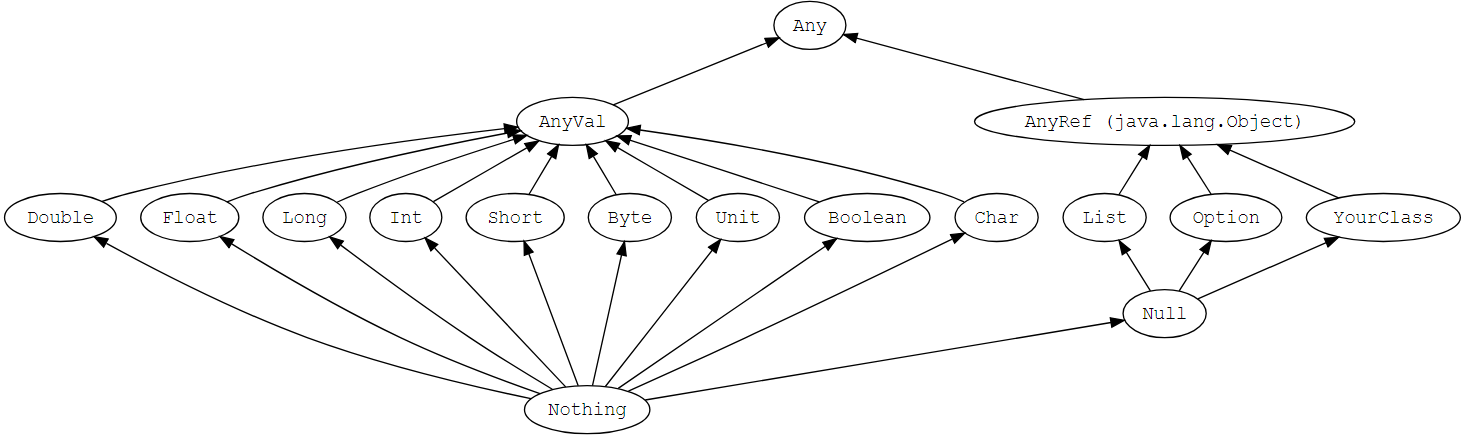
\includegraphics[width=1\textwidth]{kuvat/typehierarchy}
    \caption{Scalan luokkahierarkia}
    \label{tyyppihierarkia}
\end{figure}

Alkeistietotyyppejä kuvaavat arvoluokat \code{Byte}, \code{Short}, \code{Int}, \code{Long}, \code{Char}, \code{Float}, \code{Double}, \code{Boolean} ja \code{Unit}. Kaikki paitsi \code{Unit} vastaavat Javan vastaavia kääreluokkia. \code{Unit} on erityinen tietotyyppi, joka kuvastaa funktion tyhjää paluuarvoa. Sen voi ajatella vastaavan Javan void-avainsanaa. Merkkijonoja Scalassa kuvaa tietotyyppi \code{String}, joka on tyyppialias Javan merkkijonoa kuvaavalle tietotyypille.
\cite[Luku 5]{prorgrammingInScala3rd}

Scalan alkeistietotyypit muutetaan käännösvaiheessa primitiivityypeiksi, esimerkiksi Scalan \code{Int} käännetään 32-bittiseksi sanaksi, aivan kuten Javan \code{int}. Tämä takaa yhteensopivuuden Java-kirjastojen kanssa. Se parantaa myös suorituskykyä, sillä primitiiviarvolle ei tarvitse allokoida muistia ajon aikana.
\cite[Luku 6]{prorgrammingInScala3rd}


\section{Kontrollirakenteet}

\subsection{Ehtolauseet}
Ehtolauseita kirjoitetaan Scalassa \textit{if/else}-lausekkeiden avulla. Lauseketta voi käyttää imperatiiviseen tyyliin eli jos ehto arvioituu todeksi, suoritetaan if-lohko, muuten else-lohko.
\begin{lstlisting}
    val x = true
    if (x) {
        println("True")
    } else {
        println("False")
    }
    // Tulostaa "True"
\end{lstlisting}
Scalan if-lausekkeella on myös arvo, eli if-lauseke palauttaa arvon. Arvon palauttava if-lauseke on siis funktionaalinen, koska sillä on arvo. Esimerkiksi \codebl{val y = if (x >= 0) \"positive\" else \"negative\"} asettaa muuttujan \code{y} arvoksi joko merkkijonon "positive" tai "negative", riippuen muuttujan \code{x} arvosta. Huomattavaa on myös, että if-lauseke voidaan kirjoittaa yhdelle riville ilman aaltosulkeita. 
\cite[Luku 2.1]{scalaForTheImpatient}
        
\subsection{Silmukat}
Silmukoita Scalassa on kolmenlaisia: \code{while}, \code{do} ja \code{for}. While-silmukka suorittaa sitä seuraavaa lohkoa 0-n kertaa, kunnes annettu ehto arvioituu epätodeksi. Do-silmukka toimii vastaavalla tavalla, mutta sitä suoritetaan 1-n kertaa.
\begin{lstlisting}
    val x = false
		while (x)
			println("while")
		
		do
			println("do")
        while (x)
\end{lstlisting}
Yllä oleva esimerkki ei suorita while-silmukkaa kertaakaan, ja do-silmukan kerran.
\cite[Luku 2.5]{scalaForTheImpatient}

Scalan \code{for}-lauseke on monipuolisempi kuin monissa muissa kielissä. Sitä voi käyttää perinteiseen tapaan silmukkana, jolloin for-lausekkeen \textit{generaattori} antaa määriteltyjä arvoja yksi kerrallaan muuttujan \code{i} kautta. Lauseketta voidaan käyttää myös usean generaattorin kanssa ja arvoja voidaan suodattaa lausekkeen sisällä. Kuten if-lauseke, myös for-lauseke voi palauttaa arvon. Seuraavaksi esimerkki kummastakin käyttötavasta.
\begin{lstlisting}
    for (i <- 1 to 10)
        println(i)
\end{lstlisting}
Silmukkana lauseketta voi käyttää yllä olevan esimerkin tapaan tulostamaan kaikki numerot yhdestä kymmeneen.
\begin{lstlisting}
    val res = for {
        x <- 1 to 10
        if x % 2 == 0
    } yield (x * 2) // Vector(4, 8, 12, 16, 20)
\end{lstlisting}
Yllä olevassa esimerkissä luodaan kokonaisnumerovektori yhdestä kymmeneen, suodatetaan parilliset arvot, palautetaan jäljelle jäääneet arvot kahdella kerrottuna ja asetetaan palautettu vektori muuttujaan \code{res}. Tälläinen \code{for}-lauseke on yleinen funktionaalisessa Scalassa.
\cite[Luku 2.6]{scalaForTheImpatient}


\section{Metodit ja funktiot} \label{MetoditJaFunktiot}
Jokainen operaatio Scalassa on metodikutsu. Myös tavanomaiset aritmeettiset operaattorit on toteutettu metodikutsuina. Esimerkiksi kahden kokonaisluvun yhteenlasku \code{1 + 2} on lyhyempi versio metodikutsusta \code{1.+(2)}. Scalassa on mahdollista määritellä funktio kahdella tavalla: olion metodiksi tai funktioliteraaliksi. Metodi voidaan määritellä \code{def}-avainsanalla.
Scalassa funktio palauttaa automaattisesti viimeisen lausekkeensa arvon, joten \code{return}-avainsanan käyttö on vapaaehtoista ja sitä käytetään vain harvoin.
\cite[Luku 1.4]{scalaForTheImpatient}
\cite[Basics]{tourOfScala}

\subsection{Funktioliteraalit}
Funktioliteraali on funktio, jota käsitellään kuten mitä tahansa muuttujaa. Yleensä funktioliteraali sijoitetaan muuttujaan tai annetaan parametriksi toiselle funktiolle. Kuten muillakin muuttujilla, funktioilla ja metodeilla on Scalassa aina tyyppi. Tyypin voi määritellä eksplisiittisesti, mutta monesti Scala osaa päätellä funktion tyypin.
Seuraavassa esimerkissä määritellään kummallakin tavoilla funktio, joka kertoo onko parametrina annettu kokonaisluku parillinen. Funktion tyyppi on siis \code{Int => Boolean}.
\cite[Luku 8]{prorgrammingInScala3rd}
\begin{lstlisting}
    def isEven1(x: Int): Boolean = x % 2 == 0
    val isEven2: (Int => Boolean) = x => x % 2 == 0
\end{lstlisting}

\subsection{Korkeamman asteen funktiot}
Funktio voi ottaa parametriksi toisen funktion tai palauttaa funktion. Tälläisiä funktioita kutsutaan \textit{korkeamman asteen funktioiksi}. Korkeamman asteen funktiot ovat yksi funktionaalisen ohjelmoinnin kulmakivistä. Seuraavassa esitellään korkeamman asteen funktio, joka ottaa parametrina kokonaisluvun sekä funktion kokonaisluvusta kokonaislukuu, ja palauttaa kutsuu tätä funktiota parametrin kokonaisluvulle.
\begin{lstlisting}
    def mapValue(v: Int, m: Int => Int): Int = m(v)
    
    def double(x: Int): Int = x * 2
    
    mapValue(2, double)
    mapValue(2, _ * 3)
\end{lstlisting}
Kuten yllä olevasta esimerkistä huomataan, annetaan \code{double}-funktio parametrinä ihan kuten mikä tahansa muukin muuttuja. Esimerkin viimeisellä rivillä käytetään funktioliteraalia \code{_ * 3}, joka on lyhyempi muoto funktioliteraalille \code{x => x * 3}.
\cite[Luku 12]{scalaForTheImpatient}


\section{Luokat ja oliot} \label{LuokatJaOliot}
Scalassa on useita erilaisia luokka- ja oliotyyppejä sekä tapoja luoda instansseja luokista. Tässä luvussa esitellään pääpiirteittäin erilaiset luokkatyypit.

\subsection{Class} \label{class}
Luokka voidaan määritellä Scalassa \code{class}-avainsanalla. Luokka voi olla tyhjä tai se voi sisältää metodeita ja muuttujia. Luokasta luodaan instanssi \code{new}-avainsanalla. Luokan sisältämät kentät voidaan määritellä konstruktorissa heti luokan nimen jälkeen suluissa. Konstruktorissa määritellyt kentät ovat oletuksena \code{private val}. Luokasta saadaan uusi instanssi \code{new}-avainsanan avulla. Ihmistä kuvaava luokka ja instanssi voidaan määritellä seuraavalla tavalla:
\begin{lstlisting}
    class Person(val name: String, var age: Int) {
        def isAdult = age >= 18
    }
    val p = new Person("Matti", 30)
\end{lstlisting}
Luokassa Person on kaksi kenttää: julkinen muuttumaton kenttä nimi ja julkinen muutettava ikä. Lisäksi luokassa on metodi, joka kertoo onko henkilö täysi-ikäinen.
\cite[Classes]{tourOfScala}


\subsection{Case class} \label{caseclass}
Scalassa on myös erityisiä case-luokkia, joita käytetään yleensä kuvaamaan muuttumatonta dataa. Case-luokka määritellään kuten tavallinen luokka, mutta konstruktorissa määriteltävät kentät ovat oletuksena \code{public val}. Case-luokkaan voidaan määräitellä metodeita samoin kuin tavalliseenkin luokkaan. Case-luokan instanssia luotaessa ei tarvitse käyttää \code{new}-avainsanaa. Puhelinmallia kuvaava case-luokka ja instanssi voidaan määritellä seuraavalla tavalla:
\begin{lstlisting}
    case class Phone(brand: String, model: String)
    val p = Phone("Google", "Pixel4")
\end{lstlisting}
Scala-kääntäjä lisää case-luokkiin \code{toString}-, \code{hashCode}-, \code{equals}- ja \code{copy}-metodeita oletustoteutuksilla. Lisäksi kääntäjä lisää \textit{kumppaniolioon} \code{apply}-tehdasmetodin, jonka avulla uusien instanssien luonti tapahtuu.
\cite[Luku 15]{prorgrammingInScala3rd}

Tavallisia luokkia käytetään varsinkin oliotyylisessä ohjelmoinnissa, kun taas case-luokat ovat käytössä erityisesti funktionaalisessa Scalassa, kun halutaan käyttää muuttumattomia olioita. Tavallisten luokkien ja case-luokkien yhtäsuuruusvertailut eroavat toisistaan merkittävästi. Tavallisia luokkia verrataan viittauksen mukaan, eli osoittaako viittaus samaan olioon JVM:ssä. Case-luokkien yhtäsuuruutta verrataan olion kenttien arvon mukaan.
\cite[Luku 15]{prorgrammingInScala3rd}

\subsection{Singleton-oliot} \label{singleton-oliot}
Useat muut oliokielet tarjoavat mahdollisuuden kirjoittaa staattisia luokkia tai staattisia kenttiä luokkiin. Scalassa tälläistä staattisuutta ei ole, vaan vastaava toiminnallisuus mahdollistetaan erityisien \textit{singleton}-olioiden kautta. Singleton-oliosta on ajon aikana olemassa vain yksi instanssi, ja Scala luo sen automaattisesti. Singleton-olion on mahdollista periä luokka. Viittaaminen olioon tapahtuu yksinkertaisesti olion nimellä.
\cite[Singleton objects]{tourOfScala}

Singleton-oliota voidaan kutsua myös kumppaniolioksi, jos se on määritelty saman nimisen luokan yhteydessä. Kumppanioliot näkevät ilmentymiensä yksityiset kentät, ja ilmentymät näkevät kumppaniolionsa yksityiset kentät. Luvun \ref{caseclass} Phone-luokalle voidaan luoda kumppaniolio seuraavalla tavalla:
\begin{lstlisting}
    object Phone {
        def iphone11 = new Phone("Apple", "iPhone 11")
    }
    val iphone = Phone.iphone11
\end{lstlisting}
Tässä tapauksessa kumppanioliossa on vain yksi metodi, jonka avulla voidaan luoda helposti instansseja.
\cite[Luku 4]{prorgrammingInScala3rd}


\subsection{Piirretyypit} \label{piirretyypit}
Piirretyyppejä käytetään Scalassa määrittelemään olioiden tarjoamien palveluiden rajapintoja ja mahdollistamaan ohjelmakoodin uudelleenkäytettävyyttä. Uusi piirretyyppi luodaan \code{trait}-avainsanalla. Piirretyyppien on myös sallittua periä toisia piirretyyppejä tai luokkia. Myös singleton-olioihin on mahdollista liittää piirretyyppejä. Piirretyypin voi ajatella olevan Javan rajapintaluokan ja abstraktin luokan yhdistelmä.
\cite[Luku 6 ja 12]{prorgrammingInScala3rd}

Piirretyypin jäseniksi voidaan määritellä metodeita tai muuttujia. Jäsenet voivat olla abstrakteja tai konkreetteja. Abstraktille jäsenelle tulee toteuttavan luokan tarjota toteutus, kun taas konkreettielle jäsenille ei. Yhdessä piirreluokassa voi olla sekä abstrakteja että konkreetteja jäseniä. Tietyissä erityistapauksissa metodi voidaan merkitä abstraktiksi, vaikka sille on annettu toteutus piirretyypissä.
\cite[Luku 10]{scalaForTheImpatient}

\chapter{Kokoelmat} \label{Kokoelmat}
Tutkimuksen kohteena on Scalan standardikirjaston kokoelmat versiosta 2.8 versioon 2.12. Standardikirjastossa on toteutus useimmille yleisimmille kokoelmaluokille kuten taulukoille, listoille, joukoille(\code{Set}) ja assosiaatiotauluille(\code{Map}). Scalan kokoelmaluokat ovat paketissa \code{scala.collection}. Muuttumattomat kokoelmat ovat alipaketissa \code{immutable} ja muuttuvat alipaketissa \code{mutable}.
\cite{scalaCollections}

Muuttumattoman kokoelman sisältämät alkiot eivät voi muuttua alustamisen jälkeen. Tämä tarkoittaa, ettei alkioiden lisääminen, poistaminen tai uudelleenjärjestäminen ole mahdollista. Kokoelman muuttamista muistuttavat operaatiot, kuten \code{map}, \code{reverse}, \\\code{fold} ja kokoelmien yhdistäminen, palauttavat aina uuden kokoelman jättäen alkuperäisen kokoelman ennalleen. Käytännössä kuitenkaan aina ei kaikkia muuttumattoman kokoelman alkioita ei tarvitse kopioida, vaan tietorakenteet pyrkivät käyttämään hyväkseen rakenteellista jakamista parantaakseen suorituskykyä ja optimoidakseen muistinkäyttöä. Muuttuvissa kokoelmissa on nimensä mukaisesti mahdollista vaihtaa alkioiden järjestystä, lisätä ja poistaa alkioita kokoelmasta luomatta uutta kokoelmaa.
\cite{scalaCollections}
\cite[Luku 22]{prorgrammingInScala3rd}

Kokoelmaluokat noudattavat piirreluokkien määrittelemää hierarkiaa, joka on paketissa \code{scala.collection}. Hierarkia on sama sekä muuttumattomille että muuttuville kokoelmille. Ylimpänä hierarkiassa on \code{Traversable}-piirreluokka, jolla on yksi välitön aliluokka, \code{Iterable}. \code{Iterable}:lla on kolme välitöntä aliluokkaa \code{Seq}, \code{Set} ja \code{Map}, jotka edustavat järjestettyjä kokoelmia, joukkoja ja assosiaatiotauluja. Kuvassa \ref{kokoelmahierarkia} näytetään lisäksi vielä muutama aliluokka.
\cite{scalaCollections}
\begin{figure}[h]
    \centering\usetikzlibrary{shapes.geometric, arrows}


\tikzstyle{trait} = [rectangle, rounded corners, minimum width=2cm, minimum height=1cm,text centered, draw=black, fill=white]
\tikzstyle{arrow} = [thick,->,>=stealth]

\begin{tikzpicture}[align=center, node distance=2cm]
    \node (traversable) [trait] {Traversable};
    \node (iterable) [trait, below of=traversable] {Iterable};
    \node (set) [trait, below of=iterable] {Set};
    \node (sortedset) [trait, below of=set] {SortedSet};

    \begin{scope}[node distance=25mm]
        \node (seq) [trait, left of=set] {Seq};
        \node (linearseq) [trait, left of=sortedset] {LinearSeq};
        
        \node (map) [trait, right of=set] {Map};
        \node (sortedmap) [trait, right of=sortedset] {SortedMap};
        
        \node (indexedseq) [trait, left of=linearseq] {IndexedSeq};
    \end{scope}

    \draw [arrow] (traversable) -- (iterable);

    \draw [arrow] (iterable) -- (set);
    \draw [arrow] (iterable) -- (seq);
    \draw [arrow] (iterable) -- (map);
    
    \draw [arrow] (seq) -- (indexedseq);
    \draw [arrow] (seq) -- (linearseq);
    
    \draw [arrow] (set) -- (sortedset);

    \draw [arrow] (map) -- (sortedmap);

\end{tikzpicture}
    \caption{Kokoelmien hierarkia}\label{kokoelmahierarkia}
\end{figure}


\section{Järjestetyt kokoelmat}
Suorituskykyvertailuun valittiin muuttumattomista kokoelmista \code{List}, joka tyypillinen rekursiivinen linkitetty rakenne funktionaalisessa ohjelmoinnissa, ja \code{Vector}, jossa alkion haku indeksin mukaan on tehokkaampaa. Muuttuvista kokoelmista valittiin \code{Array}, joka on kiinteän kokoinen taulukko, \code{ArrayBuffer}, joka on dynaamisesti kasvava taulukko ja \code{ListBuffer}, joka on dynaamisesti kasvava linkitetty rakenne. Kaikki kyseiset muuttuvat tietorakenteet ovat tyypillisiä olio-ohjelmoinnissa käytettyjä tietorakenteita.

\code{List} on abstrakti luokka, joka kuvaa yhteen suuntaan linkitettyä rekursiivista muuttumatonta listaa, jolla on kaksi konkreettista toteutusta: \codebl{case class ::[B](head: B, tail: List[B])} ja \code{case object Nil}. Epätyhjää listaa kuvaavassa luokassa \code{::} on kaksi jäsentä: alkio, jota kutsutaan listan \textit{pääksi}, ja \textit{häntä} joka kuvaa listan muita alkioita. Tyhjää listaa ja samalla listan loppumista kuvaa singleton-olio \code{Nil}. \code{Nil} perii luokan \code{List[Nothing]}, jolloin saman olion on mahdollista kuvata minkä tahansa listan viimeistä alkiota. Esimerkiksi luvut 1 ja 2 sisältävä lista voidaan ilmaista näin: \code{1 :: 2 :: Nil}. Listan \code{head}-ja \code{tail}-operaatiot sekä listan alkuun lisääminen tapahtuvat vakioajassa. Aikakompleksisuus alkion hakemiselle indeksin perusteella on lineaarinen.
\cite{scalaAPI}
\cite{scalaCollections}

\code{Vector} on taulukon ominaisuuksia jäljittelevä muuttumaton tietorakenne, joka on toteutettu puurakenteena, jonka solmut ovat korkeintaan 32-alkioisia taulukoita. Lehtisolmujen taulukot sisältävät vektorin varsinaisia alkioita, ja muut solmut sisältävät alemman tason taulukoita. Jos esimerkiksi alustetaan uusi 70-alkioinen vektori, on se kolmen taulukon puu, jossa juurisolmuna olevalla taulukolla on kolme lapsitaulukkoa, joista kahdessa on 32 alkiota ja yhdessä 6 alkiota. Tämä mahdollistaa taulukoiden rakenteellisen jakamisen eri vektori-instanssien kesken, mikä vähentää kopioimista ja muistinkäyttöä. Satunnaisten haku-, muokkaus- ja poisto-operaatioiden aikakompleksisuus on log(32, N), eli operaatioiden voidaan ajatella tapahtuvan lähes vakioajassa.
\cite{scalaCollections}
\cite[Luku 4]{highPerformanceProgramming}

\code{Array} on Scalassa erityinen kokoelma, joka mahdollistaa primitiivityyppisten, viittaustyyppisten ja geneeristen alkioiden tallentamisen. Primitiivityyppisiä alkioita käsitellään ilman alkioiden käärimistä olioiksi. Esimerkiksi kokonaislukuja sisältävä \\\code{Array[Int]} kääntyy Javan \code{int[]}-taulukoksi. Kuten Javassa, taulukon koko ei voi muuttua alustamisen jälkeen. Verrattuna Javan taulukoihin \code{Array} tarjoaa kuitenkin huomattavasti enemmän operaatioita. Haku- ja muokkausoperaatiot tapahtuvat vakioajassa. Häntäoperaatio vie kuitenkin lineaarisen ajan, sillä jokainen alkio, pois lukien ensimmäinen, joudutaan kopioimaan uuteen taulukkoon.
\cite{scalaCollections}

\code{ArrayBuffer} on dynaamisesti kasvava listarakenne, joka käyttää alkioiden tallentamiseen taulukkoa. Tästä johtuen useimmat operaatiot vastaavat aikakompleksisuudeltaan \code{Array}:ta. Lisäksi \code{ArrayBuffer} mahdollistaa alkion lisäämisen taulukon alkuun, loppuun sekä keskelle. Alkuun ja keskelle lisäämisen aikakompleksisuus on lineaarinen. Muut operaatiot tapahtuvat pääasiassa vakioajassa, poislukien täyteen taulukkoon lisääminen, joka vie lineaarisen ajan.
\cite{scalaCollections}

\code{ListBuffer} on dynaamisesti kasvava muuttuva kokoelma, joka on toteutettu linkitettynä rakenteena. Poiketen \code{List}:stä, \code{ListBuffer} mahdollistaa alkioiden lisäämisen rakenteen alkuun ja loppuun vakioajassa. Satunnaisen alkion haku- ja muokkausoperaatiot sekä rakenteen keskelle lisääminen ovat aikakompleksisuudeltaan lineaarisia. Myös häntäoperaatio vie lineaarisen ajan, sillä kaikki hännän alkiot täytyy kopioida uuteen tietorakenteeseen.
\cite{scalaCollections}


\section{Suorituskykyvertailut}
Tutkielmassa on käytetty kokoelmien suorituskykymittauksia kahdesta eri lähteestä: Toby Hobsonin\cite{hobsonBenchmark} ja Li Haoyi:n\cite{haoyiBenchmark} mittauksista. Järjestettyjen kokoelmien tapauksessa kiinnostuksen kohteena on yleisimpien operaatioiden suorituskyky: kokoelman luominen, iterointi, alkion satunnainen haku sekä lisääminen ja häntäoperaatio. 

Hobson\cite{hobsonBenchmark} on käyttänyt mittauksien toteutuksessa OpenJDK-tiimin kehittämää \textit{Java Microbenchmark Harness:ia} (JMH), joka sisältää useita työkaluja suorituskykymittausten tekemistä varten. Yhden testausiteraation aikana testataan 1000-alkioinen kokoelma. Jokaista mittausta varten on viisi JVM-instanssia, joita jokaista lämmitetään kymmenen iteraation verran, ja itse mittaus sisältää kymmenen iteraatiota. Mittausten yksikkönä on operaatioiden määrää sekunnissa (ops/s), jolloin suuri luku tarkoittaa hyvää suorituskykyä.
\cite{highPerformanceProgramming}

Haoyi ei käytä mittauksissaan\cite{haoyiBenchmark} JMH:ta. Suorituskykyä on mitattu eri kokoisilla kokoelmilla, ja kaavioihin on valittu kyseisen operaation kannalta mielekkäät koot kokoelmille. Ennen jokaista yksittäistä mittausta pakotetaan virtuaalikoneen roskien keräys, ja virtuaalikonetta lämmitetään ajamalla yksi iteraatio mittausta, jonka jälkeen tehdään itse mittaus. Yksi mittauskierros sisältää yhden mittauksen jokaiselle kokoelman ja koon yhdistelmälle. Kaikki mittaukset sisältäviä mittauskierroksia tehdään yhteensä seitsemän kappaletta, joista lasketaan keskiarvo. Mittausten yksikkö on operaation suorittamiseen kuluva aika nanosekunneissa, eli pieni arvo tarkoittaa hyvää suorituskykyä. 


\subsection{Iterointi}
Iteroinnissa kokoelman jokainen alkio käydään läpi. Operaation oletettu aikakompleksisuus on lineaarinen. Iterointioperaatio ei muokkaa iteroitavaa kokoelmaa, joten muuttuvien ja muuttumattomien kokoelmien suorituskyvyissä ei pitäisi olla merkittäviä eroja. Lähteenä käytettävissä suorituskykymittauksissa ei tutkittu rinnakkaisten kokoelmien suorituskykyä, joten iterointi tapahtui järjestyksessä.

Haoyin mittauksissa\cite{haoyiBenchmark} \code{Array}:n iteroiminen \code{while}-silmukalla sekä \\\code{ArrayBuffer}:n iteroiminen tapahtui mittaamattoman lyhyessä tai jopa negatiivisessa ajassa, joten on kyseisiä mittauksia ei otettu huomioon. Kaaviosta \ref{iterointi_kaavio} voidaan huomata, että suorituskyvyissä ei ollut suuria eroavaisuuksia, paitsi Hobsonin mittauksissa\cite{hobsonBenchmark} \code{ArrayBuffer} oli 3-4 kertaa muita kokoelmia nopeampi. Haoyin mittauksissa\cite{haoyiBenchmark} merkittävää eroa ei ollut, vaikkakin \code{Array} oli hieman muita nopeampi.

\begin{figure}[h]
    \centering
    \definecolor{list}{HTML}{4F81BD}
\definecolor{vector}{HTML}{C0504D}
\definecolor{array}{HTML}{00FF00}
\definecolor{arraybuffer}{HTML}{9F4C7C}
\definecolor{listbuffer}{HTML}{FCBA03}

\pgfplotstableread{
    size    List    Vector  Array
    4096    14100   16200   14200
    16192   55000   62000   55600
    65536   231000  256000  228000
    262144  920000  1030000 910000
}\haoyi

\pgfplotstableread{
    collection  result
    List        396586
    Vector      321700
    Array       1226833
    ArrayBuffer 412568
    ListBuffer  3434340
}\hobson

\begin{tikzpicture}
    \begin{axis}[
        width=0.52*\textwidth,
        xshift=-2cm,
        xtick=data,
        xticklabels from table={\haoyi}{size},
        ymin=0,
        name={haoyi},
        title={Haoyi},
        xlabel={Kokoelman koko},
        legend pos=north west,
        legend style={draw=none},
    ]

    \addplot+[blue] table [y=List, x expr=\coordindex]{\haoyi};
    \addplot+[red] table [y=Vector, x expr=\coordindex]{\haoyi};
    \addplot+[green] table [y=Array, x expr=\coordindex]{\haoyi};

    \legend{List, Vector, Array, ArrayBuffer}

    \end{axis}

    \begin{axis}[
        at={(haoyi.south east)},
        xshift=1cm,
        width=0.52*\textwidth,
        ybar,
        ymin=0,
        xtick=data,
        xticklabel style={rotate=45, anchor=north east},
        title={Hobson},
        symbolic x coords={List, Vector, Array, ArrayBuffer, ListBuffer}
    ]
    
    \addplot table[x=collection, y=result]{\hobson};

\end{axis}

\end{tikzpicture}
    \caption{Iterointi}\label{iterointi_kaavio}
\end{figure}


\subsection{Satunnainen haku}
Nimensä mukaan satunnainen haku tarkoittaa alkion hakemista kokoelmasta satunnaisen indeksin perusteella. Linkitetyissä rakenteissa haku vaatii alkioiden käymistä läpi peräkkäin, kunnes haettu indeksi saavutetaan, jolloin aikakompleksisuus on lineaarinen. Taulukkopohjaisissa tietorakenteissa vastaavaa rajoitetta ei ole, vaan alkion muistiosoite voidaan laskea suoraan indeksin perusteella ja haun voi olettaa tapahtuvan vakioajassa. Tästä syystä on perusteltua olettaa taulukkojen olevan huomattavasti linkitettyjä rakenteita suorituskykyisempiä.

Hobsonin mittaukset\cite{hobsonBenchmark} kaaviossa \ref{satunnainenHaku_kaavio} tukevat tätä hypoteesia. \code{ListBuffer} sekä \code{List} ovat jopa useita satoja kertoja hitaampia kuin taulukoihin pohjautuvat kokoelmat. Hieman yllättäen \code{ListBuffer} on kuitenkin noin 3,5 kertaa nopeampi kuin \code{List}, vaikka \code{ListBuffer} käyttää sisäisesti alkioiden tallentamiseen \code{List}:iä. Taulukon ominaisuuksia mukaileva \code{Vector} ja \code{Array} olivat suorituskyvyltään lähes identtisiä. \\\code{ArrayBuffer} oli noin 15 \% nopeampi kuin muut taulukkopohjaiset kokoelmat, mikä on hieman yllättävää, sillä sisäisesti alkiot tallennetaan käyttäen \code{Array}:ta.

\begin{figure}[h]
    \centering
    \pgfplotstableread{
    collection  result
    List        313253
    Vector      62082283
    Array       60777210
    ArrayBuffer 72734680
    ListBuffer  1107126
}\hobson

\begin{tikzpicture}
    \begin{axis}[
        at={(haoyi.south east)},
        ybar,
        width=12cm,
        height=9cm,
        ymin=0,
        xtick=data,
        title={Hobson},
        ylabel={ops/s},
        symbolic x coords={List, Vector, Array, ArrayBuffer, ListBuffer},
        nodes near coords,
        every node near coord/.append style={/pgf/number format/fixed},
    ]
    
    \addplot table[x=collection, y=result]{\hobson};

\end{axis}

\end{tikzpicture}
    \caption{Satunnainen haku}\label{satunnainenHaku_kaavio}
\end{figure}


\subsection{Kokoelman luominen}
Kokoelmia rakennetaan useasti lisäämällä alkioita yksi kerrallaan kokoelmaan. Joskus kokoelma luodaan toisen kokoelman tai kokoelmatyypin alkioista. Taulukkoja (Scalassa \code{Array}) luodessa täytyy yleensä päättää, miten suuri taulukko luodaan. Mikäli täyteen taulukkoon halutaan lisätä alkioita, täytyy luoda uusi suurempi taulukko ja kopioida kaikki alkiot alkuperäisestä taulukosta uuteen taulukkoon ja lisätä uusi alkio uuteen taulukkoon. Tästä syystä taulukon luominen alkio kerrallaan johtaa neliölliseen aikakompleksisuuteen.

Haoyin vertailuissa\cite{haoyiBenchmark} (kaavio \ref{kokoelmanLuominen_kaavio}) on testattu useita tapoja kokoelmien luomiseen. \code{Array:+} kuvastaa tilannetta, jossa luodaan kokoelma lisäämällä alkio täyteen taulukkoon. Oletetusti sen suorituskyky on koko vertailun huonoin. \code{Array}-prealloc kuvaa tilannetta, jossa luodaan valmiiksi oikean kokoinen taulukko, ja sen suorituskyky on vertailun paras.

\code{List::} rakentaa linkitetyn rakenteen lisäämällä alkioita linkitetyn listan alkuun, eli alkio lisätään \code{::}-olion pääksi ja hännäksi lisätään lista. Operaation aikakompleksisuus on vakio. \cite{scalaCollections} Hayoin mittaukset osoittavat tämän todeksi, ja ainoastaan \code{Array}-prealloc oli \code{List}:aa suorituskykyisempi.

Kun \code{ArrayBuffer}:n sisäinen taulukko tulee täyteen, luodaan uusi, kaksi kertaa alkuperäistä suurempi, taulukko ja vanhan taulukon arvot kopioidaan uuteen. Valtaosa lisäyksistä tapahtuu vakioajassa, mutta lisäys sisäisen taulukon ollessa täysi vie lineaarisen ajan. Suorituskyky on odotetusti linkitettyä rakennetta huonompi, mutta hieman \code{Array.toVector}:ia parempi.

\code{Vector:+} aikakompleksisuuden ilmoitetaan olevan käytännössä vakio \cite{scalaCollections}, mutta vakion voi olettaa olevan suurempi kuin \code{ArrayBuffer}:lla, sillä osa puurakenteen solmuista joudutaan kopioimaan.  Suurempi vakiokerroin näkyy mittauksissa selvästi. Erityisesti luotaessa yli suuria kokoelmia, kasvaa kopioinnin tarve, kun sisäiseen puurakenteeseen lisää tasoja. Mittauksissa suorituskyky heikkenee merkittävästi yli 1024 alkion kokoelmissa.

Suorituskykyisempi tapa luoda \code{Vector} on luoda toinen kokoelma ja kutsua sen \code{toVector}-metodia. Haoyin\cite{haoyiBenchmark} mittausten \code{Array.toVector} on tilanne, jossa luodaan \code{Array} pre-alloc-tyylisesti ja luodaan sen pohjalta \code{Vector}. Suorituskyky on huomattavasti parempi kuin lisäämällä alkioita yksi kerrallaan.

\begin{figure}[h]
    \centering
    \pgfplotstableread{
    size    List::  Vector:+ Array.toVector Array:+ Array-prealloc  ArrayBuffer
    64      301     1730     903            1460    186             691
    1024    4900    28600    12850          260000  2710            10840
    4096    19800   324000   51100          3170000 11000           43000
}\haoyi

\begin{tikzpicture}
    \begin{axis}[
        width=12cm,
        height=9cm,
        xtick=data,
        xticklabels from table={\haoyi}{size},
        ymin=0,
        ymax=55000,
        name={haoyi},
        title={Haoyi},
        ylabel={ns},
        xlabel={Kokoelman koko},
        legend pos=north west,
        legend style={draw=none},
    ]

    \addplot+[blue] table [y=List::, x expr=\coordindex]{\haoyi};
    \addplot+[red] table [y=Vector:+, x expr=\coordindex]{\haoyi};
    \addplot+[violet] table [y=Array.toVector, x expr=\coordindex]{\haoyi};
    \addplot+[green] table [y=Array:+, x expr=\coordindex]{\haoyi};
    \addplot+[black] table [y=Array-prealloc, x expr=\coordindex]{\haoyi};
    \addplot+[brown] table [y=ArrayBuffer, x expr=\coordindex]{\haoyi};

    \legend{List::, Vector:+, Array.toVector, Array:+, Array-prealloc, ArrayBuffer}

    \end{axis}

\end{tikzpicture}
    \caption{Kokoelman luominen}\label{kokoelmanLuominen_kaavio}
\end{figure}


\begin{figure}[h]
    \centering
    \definecolor{list}{HTML}{4F81BD}
\definecolor{vector}{HTML}{C0504D}
\definecolor{array}{HTML}{00FF00}
\definecolor{arraybuffer}{HTML}{9F4C7C}
\definecolor{listbuffer}{HTML}{FCBA03}

\pgfplotstableread{
    collection              result
    List                    307
    List(prepend)           39799
    Vector                  26882
    Array*                  49790
    ArrayBuffer             173677
    ListBuffer              69692
    ListBuffer(prepend)     39799
}\hobson

% "As you can see in the source, I actually allocated a 1000 element array then copied each element into the slot so it’s not strictly an append operation."

\begin{tikzpicture}
    \begin{axis}[
        at={(haoyi.south east)},
        ybar,
        width=12cm,
        height=9cm,
        ymin=0,
        xtick=data,
        title={Hobson},
        symbolic x coords={List, List(prepend), Vector, Array*, ArrayBuffer, ListBuffer, ListBuffer(prepend)},
        xticklabel style={rotate=45, anchor=north east},
    ]
    
    \addplot table[x=collection, y=result]{\hobson};

\end{axis}

\end{tikzpicture}
    \caption{Kokoelman loppuun lisääminen}\label{kokoelmanLoppuunLisaaminen_kaavio}
\end{figure}

\subsection{Kokoelman loppuun lisääminen}
Asetelma Hobsonin mittauksessa\cite{hobsonBenchmark} kokoelman loppuun lisäämisestä on hieman samankaltainen kuin Haoyin\cite{haoyiBenchmark} kokoelman luomisen mittauksessa. Muuttumattoman linkitetyn listan (\code{List}) tapauksessa täytyy jokainen alkio kopioida uuteen kokoelmaan ja uusi alkio lisätä juuri luodun kokoelman viimeiseksi. Operaation aikakompleksisuus on lineaarinen. Kaaviosta \ref{kokoelmanLoppuunLisaaminen_kaavio} voidaan huomata, että suorituskyky on selvästi vertailun heikoin.

\code{List}-prepend tarkoittaa tilannetta, jossa alkio lisätään rakenteen alkuun, ja kokoelman järjestys käännetään. Tällä tavoin suorituskyky on jopa yli 100 kertaa parempi. Parannus suorituskyvyssä on hieman yllättävä, sillä järjestyksen kääntävän operaation aikakompleksisuus on vakio. Eroa saattaisi selittää \code{reverse}-metodin toteutus, jossa käytetään while-silmukkaa, kun taas \code{:+}-metodissa käytetään erityistä \code{CanBuildFrom}-oliota.

Muuttuvasta linkitetystä rakenteesta, \code{ListBuffer}:sta on mittaus kummallakin edellisessä kappaleessa mainitulla tavalla. Suoraan kokoelman loppuun lisäämisellä saavutetaan paras suorituskyky, ja se on jopa yli 70 \% parempi kuin lisäämällä alkuun ja kääntämällä kokoelman järjestys. Prepend-tyylillä suorituskyky on identtinen \code{List}-prepend kanssa. 

Taulukoista \code{ArrayBuffer} suoriutuu selvästi parhaiten ollen yli kolme kertaa parempi kuin seuraavaksi paras taulukkorakenne \code{Array}, vaikka kyseisessä mittauksessa luodaan valmiiksi oikean kokoinen \code{Array}. Tulos on yllättävä, sillä tuloksien voisi olettaa olevan lähes identtisiä. Mittauksen \cite{hobsonBenchmark} toteutuksessa on käytetty \code{Array.zipWithIndex}-metodia, joka muuttaa \code{Array}:n \code{WrappedArray}:ksi. Tämä voisi osaltaan selittää tulosta.

Aikaisemman testin tavoin \code{Vector} suoriutuu tästäkin mittauksesta huonommin kuin muut taulukkomaiset kokoelmat ollen noin 85 \% huonompi kuin \code{ArrayBuffer}. Syynä lienee kopioinnin tarve jokaisen alkion lisäämisen yhteydessä.


\subsection{Häntäoperaatio}
Häntäoperaatio palauttaa kokoelman, jossa on kaikki paitsi ensimmäinen alkio. Muuttuvissa kokoelmissa tämä pakottaa yleensä kopioimaan kokoelman hännän uuteen kokoelmaan, jolloin aikakompleksisuus on lineaarinen. Muuttumattomissa kokoelmissa kopioimista voidaan vähentää tai jopa välttää kokonaan hyödyntämällä rakenteellista jakamista. Muuttumattoman \code{List}:n häntäoperaation aikakompleksisuus on vakio, sillä linkitetyn rakenteen häntään saadaan viittaus yksinkertaisesti palauttamalla ensimmäisen alkion seuraaja. \code{Vector}:n häntäoperaation aikakompleksisuudeksi ilmoitettu on käytännössä vakio\cite{scalaCollections}, vaikka todellisuudessa joitain alkioita täytyy kopioida.

Haoyin\cite{haoyiBenchmark} häntäoperaation suorituskykyä mittaavassa tutkimuksessa aloitetaan n-kokoisesta kokoelmasta ja tehdään häntäoperaatiota jäljelle jäävälle kokoelmalle, kunnes jäljellä on tyhjä kokoelma. Mittauksen tulos on kulunut aika, jolloin pieni arvo tarkoittaa hyvää suorituskykyä. Kaaviossa \ref{hantaoperaatio_kaavio} on mittauksen tulokset.

\code{List} suoriutuu mittauksissa oletetusti parhaiten. \code{ArrayBuffer} suoriutui varsin yllättäen vain hieman \code{List}:iä huonommin, vaikka aikakompleksisuuden voisi olettaa olevan lineaarinen. \code{Vector} suoriutui edellä mainittuja kokoelmia huomattavasti huonommin.

Selvästi huonoiten suoriutui kuitenkin \code{Array}. Tulos on oletettu, sillä jokaisella häntäoperaatiolla kaikki paitsi taulukon ensimmäinen alkio täytyy kopioida uuteen taulukkoon. \code{Vector} on hieman \code{Array}:ta parempi, mutta sen suorituskyky on 256 alkion kokoelmalla jo noin 20 kertaa huonompi kuin kahdella suorituskykyisimmällä kokoelmalla.

\begin{figure}[h]
    \centering
    \pgfplotstableread{
    size    List    Vector  Array   ArrayBuffer
    16      21      425     582     43
    64      100     1970    4517    166
    256     420     11800   55500   630
    1024    2100    58400   82100   2510
}\haoyi

\begin{tikzpicture}
    \begin{axis}[
        width=12cm,
        height=9cm,
        xtick=data,
        xticklabels from table={\haoyi}{size},
        ymin=0,
        ymax=4000,
        title={Haoyi},
        ylabel={ns},
        xlabel={Kokoelman koko},
        legend pos=north east,
        legend style={draw=none},
    ]

    \addplot+[blue] table [y=List, x expr=\coordindex]{\haoyi};
    \addplot+[red] table [y=Vector, x expr=\coordindex]{\haoyi};
    \addplot+[green] table [y=Array, x expr=\coordindex]{\haoyi};
    \addplot+[violet] table [y=ArrayBuffer, x expr=\coordindex]{\haoyi};

    \legend{List, Vector, Array, ArrayBuffer}
\end{axis}
\end{tikzpicture}
    \caption{Häntäoperaatio}\label{hantaoperaatio_kaavio}
\end{figure}


\section{Johtopäätökset}
Iteroinnissa kaikki kokoelmat suoriutuivat verrattain tasavertaisesti, pois lukien \\\code{ArrayBuffer}:n loistava suorituskyky muihin verrattuna. Muiden kokoelmien välistä vaihtelua iteroinnin suorituskyvyssä saattaisi selittää esimerkiksi kääreluokan käyttö \code{Array}:n yhteydessä tai \code{Vector}:n puumainen rakenne, joka johtaa muutamaan epäsuoraan viittaukseen.

Satunnaisessa haussa taulukkopohjaiset kokoelmat olivat odotetusti suorituskykyisempiä kuin linkitetyt rakenteet, riippumatta siitä oliko kyseessä muuttuva vai muuttumaton kokoelma. Taulukkopohjaisten kokoelmien välisiä eroja selittää mahdollisesti alkioiden löytymättömyys prosessorin välimuistista, jota todennäköisesti tapahtuu enemmän puumaisesti toteutetun \code{Vector}:n kohdalla kuin taulukkona toteutetussa \code{ArrayBuffer}:ssa.

Kokoelman luomisen ja loppuun lisäämisen suorituskyvyissä oli huomattavia eroja riippuen käytettävästä metodista. Taulukkopohjaisen kokoelman luominen \code{:+}-metodin avulla oli \code{Array}:n tapauksessa satoja kertoja hitaampaa kuin muilla tavoilla. Käyttötarkoitukseen sopivan kokoelman ja operaation valitsemisen merkitys on siis todella merkittävä.

Myöskään häntäoperaation suorituskyvyssä muuttuvien ja muuttumattomien kokoelmien välille ei muodostunut merkittävää eroa \code{List}:n ja \code{ArrayBuffer}:n suoriutuessa hyvin sekä \code{Array}:n ja \code{Vector}:n suoriutuessa heikommin. 

Muuttumattomista kokoelmista \code{List} tarjoaa hyvän suorituskyvyn, kunhan tarvetta satunnaiselle haulle tai kokoelman loppuun lisäämiselle ei ole. \code{Vector} puolestaan tarjoaa hyvän suorituskyvyn satunnaisessa haussa, mutta häntäoperaatiota tulisi välttää sekä kokoelman rakentamiseen täytyy kiinnittää huomiota. Muuttuviin taulukkokokoelmiin verrattuna erityisesti loppuun lisäämisen ja kokoelman luomisen suorituskyvyssä joudutaan maksamaan pientä hintaa muuttumattomuudesta.

Kokonaisvaltaisesti parhaan suorituskyvyn tarjoaa muuttuva \code{ArrayBuffer}, joka suoriutuu kaikista operaatioista loistavasti, poislukien kokoelman luominen, jossa suorituskyky on keskinkertainen. Muuttuva linkitetty rakenne \code{ListBuffer} suoriutuu yleisesti hieman paremmin kuin vastaava muuttomaton kokoelma \code{List}, mutta ero on pieni.

Tutkielmassa käytettyjen lähteiden perusteella ei noussut esiin säännönmukaisia eroavaisuuksia muuttuvien ja muuttumattomien kokoelmien suorituskyvystä. Kuhunkin käyttötarkoitukseen sopivan kokoelman valitseminen on suorituskyvyn kannalta todella tärkeää. Pahimmillaan käyttötarkoitukseen epäoptimaalisen kokoelman valinta voi johtaa yli sata kertaa huonompaan suorituskykyyn verrattuna käyttötarkoitukseen sopivaan kokoelmaan.

\chapter{Yhteenveto} \label{Yhteenveto}
Tutkielmassa pyrittiin selvittämään funktionaalisen ohjelmointiparadigman vaikutuksia suorituskykyyn verrattuna imperatiiviseen paradigmaan. Vaikutuksia suorituskykyyn pyrittiin tarkastelemaan vertailemalla järjestettyjen muuttuvien ja muuttumattomien kokoelmaluokkien suorituskykyjä toisiinsa. Suorituskykyä tarkasteltiin tutustumalla lähteenä käytettyihin suorituskykymittauksiin. Tarkasteluun valittiin kullekin paradigmalle tyypillisiä kokoelmaluokkia. Johtopäätöksiä kokoelmaluokkien suorituskyvystä tehtiin vertailemalla lähteiden mittauksien tuloksia. 

Selviä eroja muuttuvien ja muuttumattomien kokoelmien suorituskyvylle ei havaittu, vaikkakin muuttuvat kokoelmat näyttäisivät suoriutuvan useissa operaatioissa hieman muuttumattomia paremmin. Suorituskyvyn kannalta tärkein tekijä oli kuitenkin kuhunkin käyttötarkoitukseen sopivan tietorakenteen valinta. Tarkempien säännönmukaisuuksien selvittämiseksi tulisi mittauksia tehdä useamman kokoelmaluokan, operaation ja skenaarion yhdistelmistä. Myös järjestämättömien kokoelmien, kuten joukkojen ja assosiaatiotaulujen, suorituskykyä tulisi vertailla.

Kokonaisvaltaista johtopäätöstä funktionaalisen paradigman suorituskykyvaikutuksista imperatiiviseen paradigmaan verrattuna ei tämän tutkielman tulosten perusteella voi tehdä. Jatkotutkimuskohteena kokoelmien osalta voisi olla laiskat ja rinnakkaiset kokoelmat. Muita tutkielman tekemisen aikana esiin nousseita jatkotutkimuksen aiheita ovat hahmontunnistus, sulkeumat, funktioiden osittainen soveltaminen sekä silmukoiden ja rekursion suorituskyvyn vertailu.


\printbibliography

\begin{comment}
Create your appendix chapters with command \textbackslash appchapter\{some
name\} instead of \textbackslash chapter\{some name\} for the automagic
page counting to work!
\end{comment}

\end{document}
